\documentclass{article} % Define la clase del documento, en este caso, un artículo
\usepackage[letterpaper,margin=3cm]{geometry} % Configura el tamaño del papel y los márgenes del documento
\usepackage{graphicx} % Permite la inserción de imágenes
\usepackage[spanish]{babel}% Activar esta configuración para informes en español, ajusta el idioma del documento
\usepackage[usenames]{color} % Permite el uso de colores definidos por nombre en el documento
\usepackage{hyperref} % Habilita enlaces y referencias dentro del documento
\hypersetup{colorlinks=true, linkcolor = black, citecolor= black} % Configura el color de los enlaces y citas
\usepackage{booktabs} % Proporciona comandos para crear tablas de alta calidad
\usepackage{natbib} % Permite el uso de citas y referencias bibliográficas con diferentes estilos
\usepackage{tikz} % Permite la creación de gráficos y diagramas vectoriales directamente en LaTeX
\usepackage{float} % Para controlar la posición de los elementos flotantes, como imágenes, con la opción [H]
\usepackage{diagbox} % Permite crear celdas con líneas diagonales en tablas
\usepackage{listings} % Permite la inclusión y formateo de código fuente en el documento
\usepackage{xcolor} % Paquete para definir y usar colores en el documento
\usepackage{parskip} % Añade espacio entre párrafos en lugar de sangrías
\usepackage{fancyhdr} % Permite personalizar encabezados y pies de página
\usepackage{amsmath} % Proporciona una amplia variedad de entornos y comandos matemáticos

\pagestyle{fancy} % Usa el estilo fancyhdr
\fancyhf{} % Borra todos los encabezados y pies de página
\renewcommand{\headrulewidth}{0pt}
\renewcommand{\footrulewidth}{0pt} % Desactiva la línea horizontal predeterminada en el pie
\setlength{\headheight}{2cm} % Ajusta la altura del encabezado para hacer espacio para la línea
\fancyhead[L]{\raisebox{0.20cm}{\textbf{Proyecto de infraestructura hidráulica}}} % Añade el texto en la parte izquierda del encabezado, subiéndolo ligeramente
\fancyhead[R]{\raisebox{0.1cm}{
\includegraphics[width=0.25\linewidth]{LOGO_UNIVERSIDAD.jpg}}} % Añade la imagen en la parte derecha del encabezado y súbela un poco
\fancyhead[C]{\rule{\textwidth}{0.6pt}} % Añade una línea horizontal superior centrada
\fancyfoot[C]{\rule{\textwidth}{0.6pt}} % Añade una línea horizontal en el pie de página centrada
\fancyfoot[R]{\raisebox{-1.5\baselineskip}{\thepage}} % Coloca el número de página a la derecha, con suficiente espacio debajo de la línea
\geometry{top=3cm, bottom=2.5cm} % Ajusta los márgenes superior e inferior

% Definición de colores al estilo Visual Studio Code
\definecolor{codegreen}{rgb}{0.25,0.49,0.48} % Comentarios
\definecolor{codegray}{rgb}{0.5,0.5,0.5} % Números y anotaciones
\definecolor{codepurple}{rgb}{0.58,0,0.82} % Palabras clave
\definecolor{backcolour}{rgb}{0.95,0.95,0.92} % Color de fondo

% Configuración del estilo de las celdas de código
\lstset{
    backgroundcolor=\color{backcolour},   % color de fondo; necesita que el paquete color o xcolor esté cargado
    commentstyle=\color{codegreen},       % estilo de comentarios
    keywordstyle=\color{codepurple},      % estilo de palabras clave
    numberstyle=\tiny\color{codegray},    % estilo de los números de línea
    stringstyle=\color{red},              % estilo de las cadenas de texto
    basicstyle=\ttfamily\small,           % estilo del texto básico
    breakatwhitespace=false,              % ajustes de líneas sólo en espacios en blanco
    breaklines=true,                      % ajustar las líneas si son muy largas
    captionpos=b,                         % posición de la leyenda (abajo)
    keepspaces=true,                      % preserva los espacios en el texto; útil si se usa monoespaciado
    numbers=left,                         % dónde poner los números de línea
    numbersep=5pt,                        % qué tan lejos están los números de línea del código
    showspaces=false,                     % mostrar espacios con subrayados particulares; reemplaza 'showstringspaces'
    showstringspaces=false,               % subrayar los espacios dentro de las cadenas solo
    showtabs=false,                       % mostrar tabulaciones en el código con subrayados particulares
    tabsize=2,                            % tamaños de tabulación a 2 espacios
    language=TeX,                         % lenguaje del código
    morecomment=[l]\#,                    % reconocer # como inicio de comentario en Python
    frame=single,                         % agregar un marco simple alrededor del código
    rulecolor=\color{black}               % color del marco
}

\begin{document}
%----------------------------------------------------------------------------------------
%   PORTADA
%Modificar desde aqui en adelante
%----------------------------------------------------------------------------------------
\begin{titlepage}%Inicio de la carátula, solo modificar los datos necesarios
\newcommand{\HRule}{\rule{\linewidth}{0.5mm}} 
\center 
%----------------------------------------------------------------------------------------
%	ENCABEZADO
%----------------------------------------------------------------------------------------

\includegraphics[width=10cm]{LOGO_UNIVERSIDAD.jpg}\\ % Si esta plantilla se copio correctamente, va a llevar la imagen del logo de la facultad.OBS: Es necesario incluir el paquete: graphicx
\vspace{3cm}
%----------------------------------------------------------------------------------------
%	SECCION DEL TITULO
%----------------------------------------------------------------------------------------
\HRule \\[0.4cm]
{ \huge \bfseries Caso 1: Central de bombeo}\\[0.4cm] % Titulo del documento
{ \huge \bfseries Proyecto de Infraestructura Hidráulica}\\[0.4cm] % Titulo del documento
\HRule \\[1.5cm]
 \vspace{5cm}
%----------------------------------------------------------------------------------------
%	SECCION DEL AUTOR
%----------------------------------------------------------------------------------------
\begin{flushright}
    { \textbf{Profesor:}\\
    Oscar Loyola\\
    \vspace{0.2cm}
    \textbf{Alumnos:}\\
    Bernardo Caprile Canala-Echevarría\\
    Pedro Valenzuela\\
    Francisco Zegers
    \vspace{0.2cm}

}
\end{flushright}
\vspace{1cm}
%----------------------------------------------------------------------------------------
%	SECCION DE LA FECHA
%----------------------------------------------------------------------------------------
{\large \textbf{\today}}\\[2cm] % El comando \today coloca la fecha del dia, y esto se actualiza con cada compilacion, en caso de querer tener una fecha estatica, reemplazar el \today por la fecha deseada
\end{titlepage}
%----------------------------------------------------------------------------------------
%  INDICE
%----------------------------------------------------------------------------------------
\newpage
\section{Resumen ejecutivo}

\newpage
\tableofcontents % Genera el índice automáticamente
\newpage
\section{Introducción}
\subsection{Objetivo}
\newpage
\section{Marco Teórico}



\newpage
\section{Desarrollo}
\subsection{Coeficiente de Manning}
Para poder obtener el coeficiente de Manning, se utilizaron los coeficientes dados en el libro Roughness Characteristics of Natural Channels-Barnes. En el cual, se encuentran fotografías de distintos tipos de cauces, y se les asigna un coeficiente de rugosidad. A continuación, se muestran las ubicaciones que más se asemejan al cauce del río Pilmaiquén junto con su respectivo coeficiente de Manning.
\begin{table}[h!]
    \centering
    \begin{tabular}{c c}
        \textbf{Ubicación} & \textbf{Coeficiente de Manning} \\
        \hline
        \textit{Clark Fork at St. Regis, Mont} & 0.028 \\ 
        \textit{Columbia River at Vernita, Wash} & 0.025 \\
        \textit{Coeur d'Alene River near Prichard, Idaho} & 0.032 \\\hline
    \end{tabular}
\end{table}
\section{Diseño de bocatoma}
El diseño de la obra de toma es una parte importante dentro del proyecto, ya que se  encarga de permitir el ingreso controlado del caudal desde el río hacia el túnel de conducción. La bocatoma capta 10 m³/s mediante una compuerta lateral.

En términos generales, la obra de toma se compone de tres elementos principales: la reja frontal, que cumple una función de protección; la compuerta de control, que regula el ingreso de agua y permite el cierre en caso de mantenimiento o emergencias; y el túnel de conducción, que transporta el caudal hacia la conducción principal.

La toma se dispone lateralmente al cauce principal, lo que permite reducir la velocidad de aproximación y minimizar el arrastre de sedimentos. La disposición lateral facilita además el mantenimiento y limpieza, ya que el flujo que ingresa a la toma es más controlado que en una entrada frontal.

En la base de la estructura se incorpora un pequeño canal de aproximación que suaviza la transición entre el flujo libre del río y el flujo dentro del túnel, este sector fue diseñado de modo que el flujo mantenga un régimen subcrítico, lo que reduce las pérdidas por turbulencia y evita cavitación.

Anterior a la compuerta se ubica la reja de protección, la cual fue diseñada considerando bajas velocidades de acercamiento para evitar el arrastre de sólidos y minimizar las pérdidas de carga. El ángulo de inclinación de la reja con respecto al flujo es un factor importante, ya que facilita la autolimpieza y reduce el impacto directo del flujo, lo que prolonga la vida útil y disminuye el riesgo de obstrucción. En este caso, la inclinación elegida permite que los residuos se desplacen hacia la superficie del río, donde pueden ser retirados manual o mecánicamente. 




\newpage
\section{Resultados}
\subsection{Dimensiones de la bocatoma}
\begin{table}
    \centering
    \begin{tabular}{c c}
        \textbf{Parámetro} & \textbf{Valor} \\
        \hline
        Caudal de diseño & 10 m$^3$/s \\ 
        Ancho de la reja & 4.0 m \\
        Velocidad en el túnel & 1.00 m/s \\
        Porosidad de la reja & 0.6 \\
        Inclinación de la reja vertical & 35 ° \\ \hline
    \end{tabular}
    \caption{Dimensiones y características principales de la bocatoma}
\end{table}

El área efectiva necesaria para el paso del caudal se determina considerando la velocidad de acercamiento y la porosidad de la reja.
De acuerdo con la siguiente ecuación:
\begin{equation}
    Q = V_a \cdot B \cdot H \cdot \phi
\end{equation}

Reemplazando valores y despejando la alturo:
\begin{equation}
    H = \frac{Q}{V_a \cdot B \cdot \phi} = \frac{10}{1.00 \cdot 4.0 \cdot 0.6} = 4.17 m
\end{equation}

Por lo tanto, la altura útil de la reja se estima en 4,2 metros, lo que representa la superficie necesaria para permitir el paso del caudal de diseño sin exceder la velocidad de entrada adoptada.

Esta altura permite un flujo controlado y garantiza que el nivel del agua en la cámara de captación se mantenga dentro de los márgenes operativos previstos.

\begin{table}
    \centering
    \begin{tabular}{c c}
        \textbf{Parámetro} & \textbf{Valor} \\
        \hline
        Ancho de la reja & 4.0 m \\
        Altura útil de la reja & 4.2 m \\ 
        Espacio entre barras de la reja & 0.1 m \\
        Espesor de las barras & 0.02 m \\
        Ángulo de inclinación & 35 ° \\
        Pérdida de carga en la reja & 0.15 m \\ \hline
    \end{tabular}
    \caption{Dimensiones finales de la bocatoma}
\end{table}

El área frontal total de la reja es de 16 m², con un área libre efectiva de 9,6 m² considerando la porosidad del 60\%.
El material propuesto es acero galvanizado de alta resistencia a la corrosión, montado sobre un marco de hormigón armado empotrado en la estructura de la toma.




Con todos los datos se procedió a ocupar el Software HEC-RAS, pero primero se ocupó los datos topográficos del terreno, para obtener los cortes transversales del río y de esta forma analizar de mejor manera el terreno. Luego, se subió esta información a HEC-RAS obteniendo lo siguiente:
\begin{figure}[h!]
    \centering
    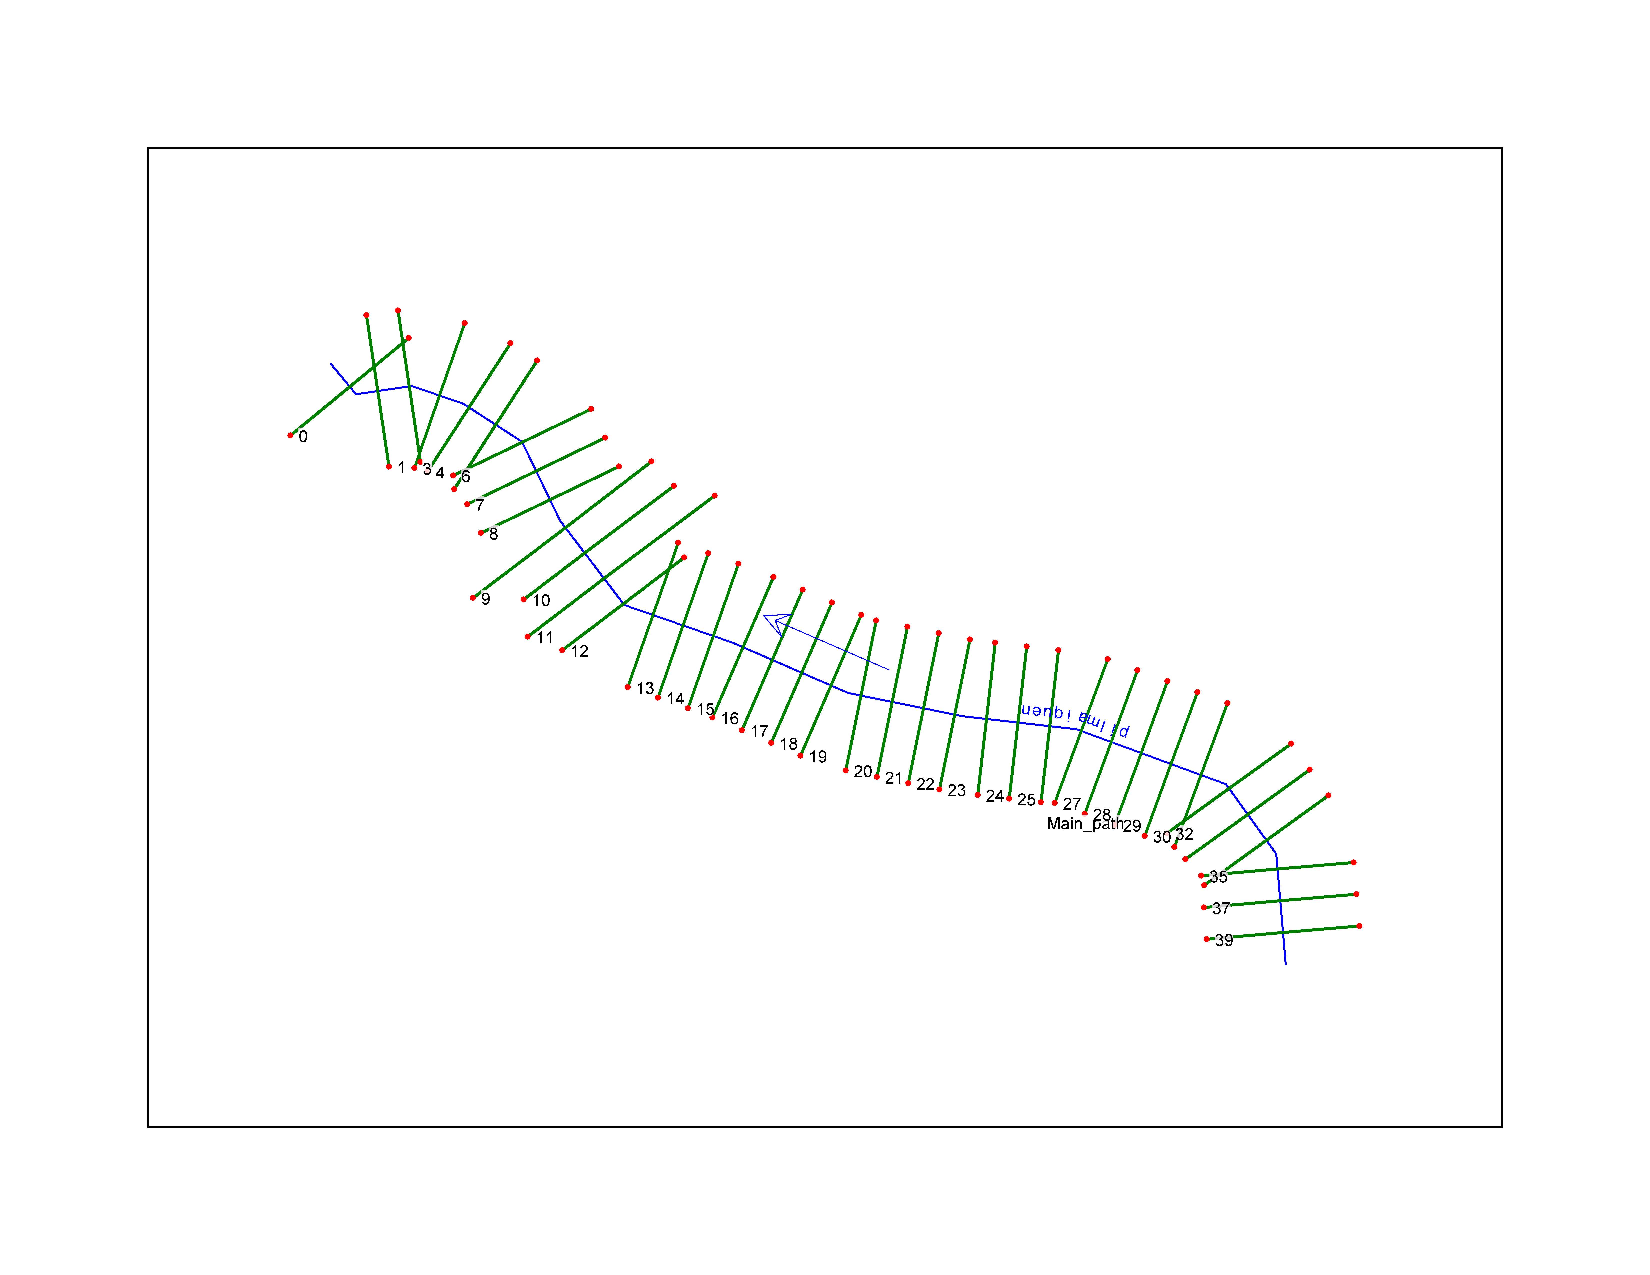
\includegraphics[width=0.6\linewidth]{imagenes/rio_sin_estruc.pdf}
    \caption{Cortes transversales del río Pilmaiquén obtenidos en HEC-RAS}
\end{figure}

Antes de empezar a incorporar al software las bocatomas y el muro se corrió con los 2 caudales asociados los periodos de retorno de categoría:

\begin{table}[h]
    \centering
    \begin{tabular}{c c}
        \textbf{Periodo de retorno (años)} & \textbf{Caudal (m$^3$/s)} \\
        \hline
        250 & 396 \\ 
        500 & 418 \\\hline
    \end{tabular}
    \caption{Caudales asociados a los periodos de retorno}
\end{table}

A continuación, se muestran los perfiles hidráulicos con los caudales anteriormente mostrados:

\begin{figure}[H]
    \centering
    \includegraphics[width=0.6\linewidth]{imagenes/perfil_250_sb.pdf}
    \caption{Perfil hidráulico con caudal asociado a periodo de retorno de 250 años}
\end{figure}

\begin{figure}[H]
    \centering
    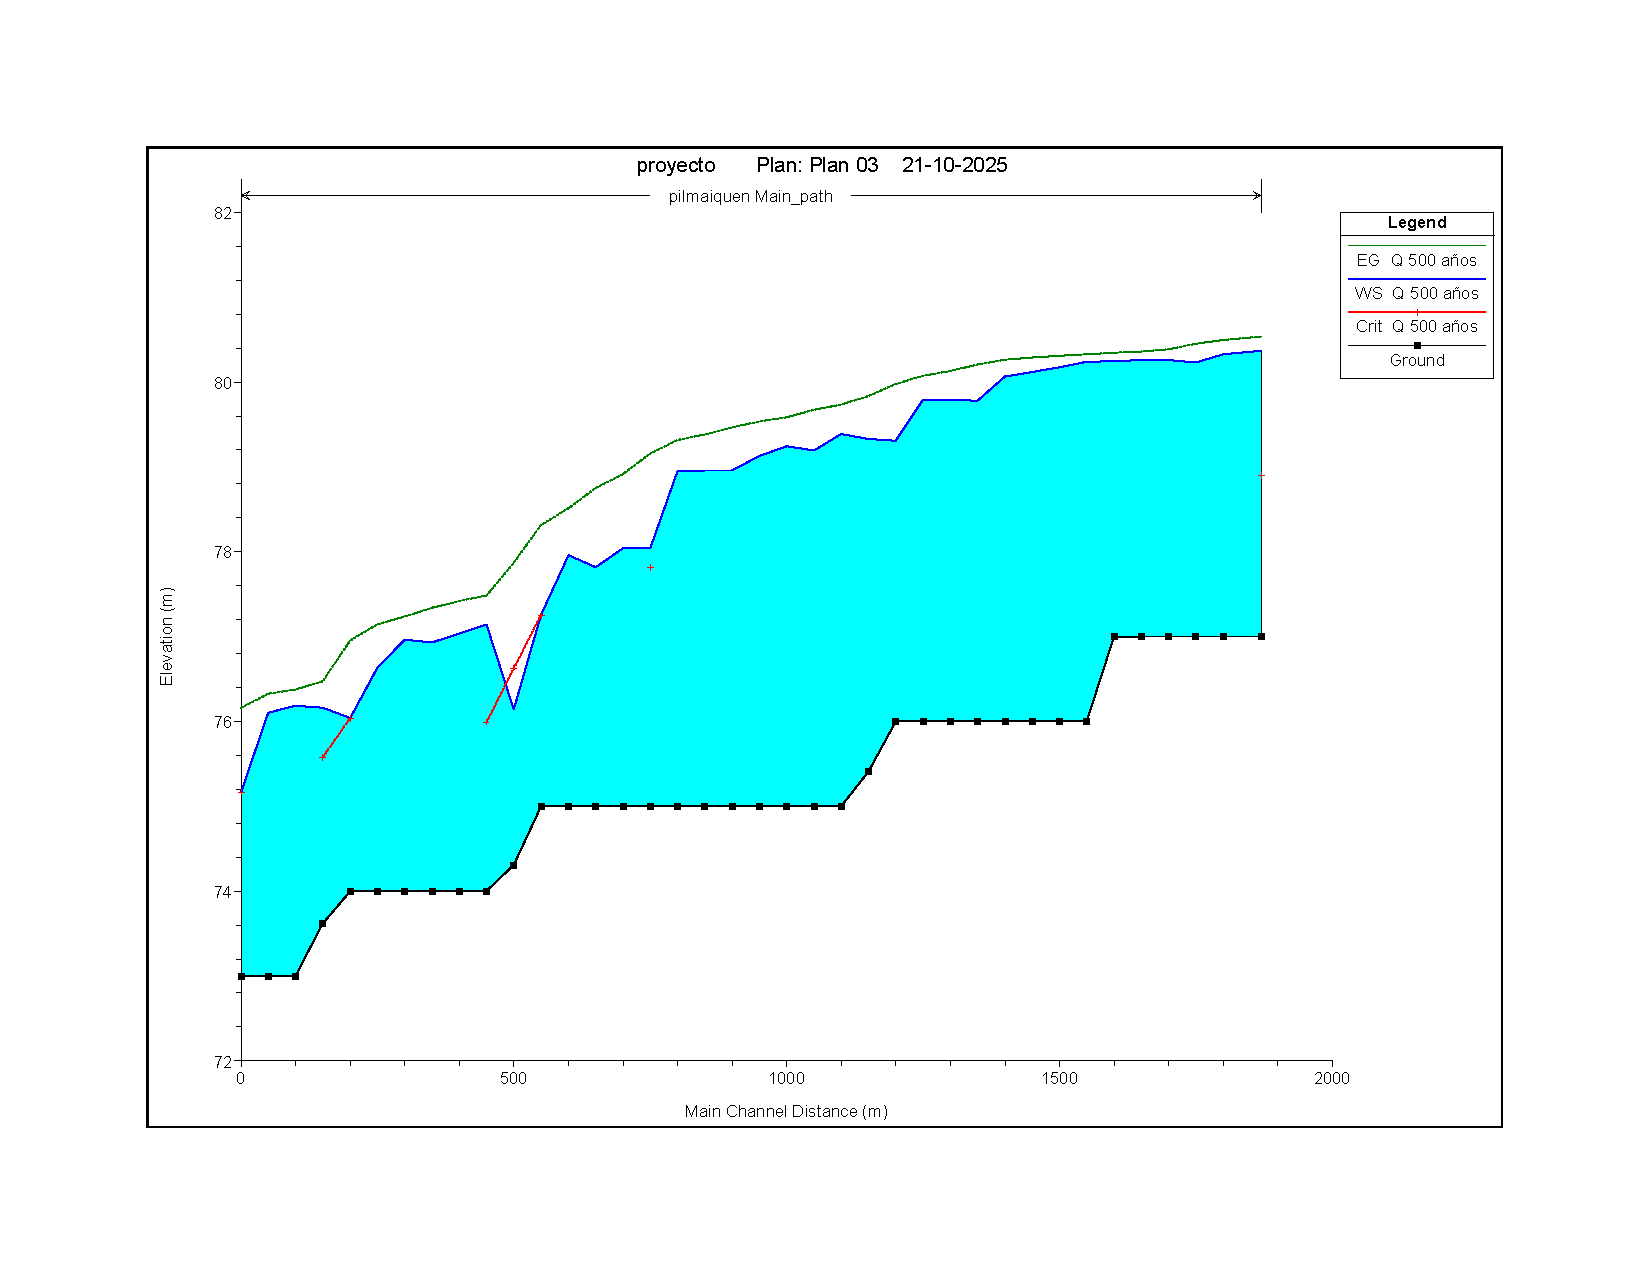
\includegraphics[width=0.6\linewidth]{imagenes/perfil_500_sb.pdf}
    \caption{Perfil hidráulico con caudal asociado a periodo de retorno de 500 años}
\end{figure}

Con los cálculos anteriormente hechos se puede empezar a dimensionar el muro con las compuertas, que se vería de la siguiente manera:

\begin{figure}[H]
    \centering
    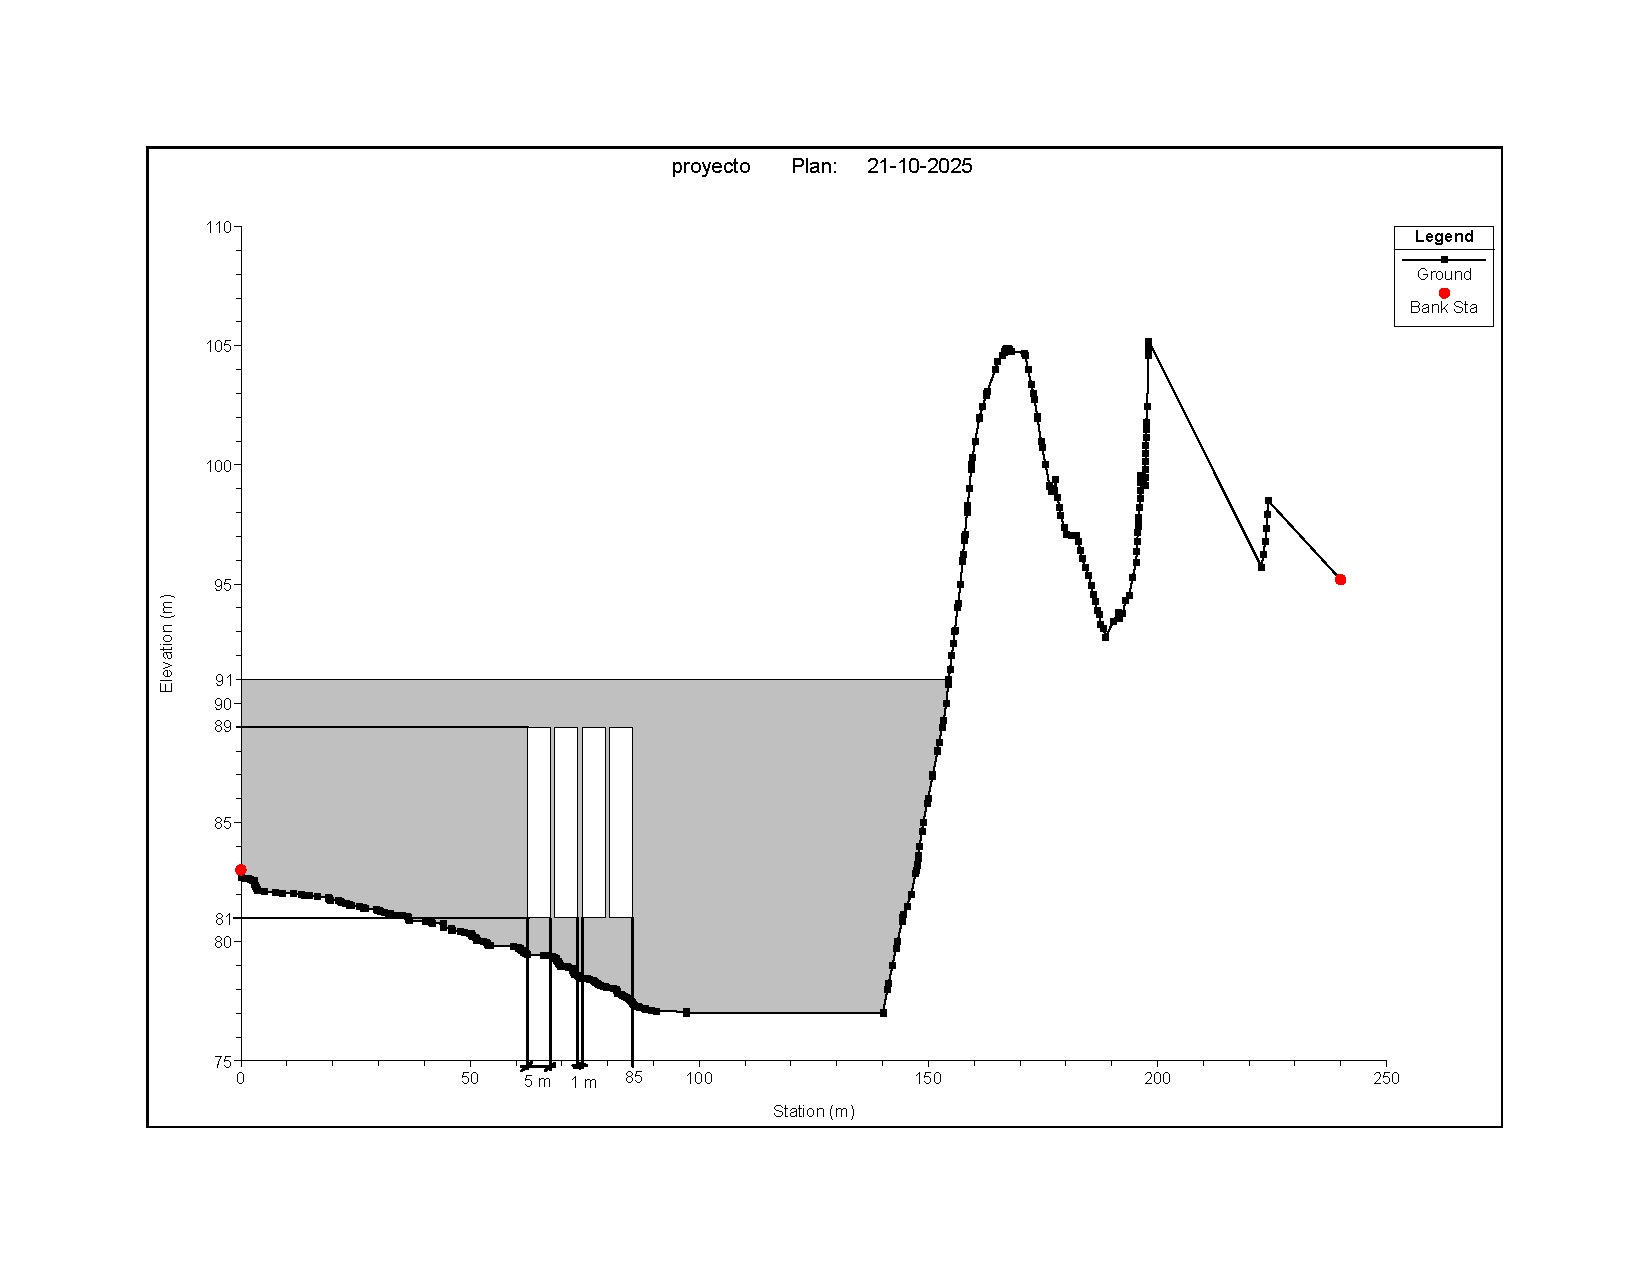
\includegraphics[width=0.8\linewidth]{imagenes/muro.pdf}
    \caption{Muro con bocatomas incorporadas al cauce del río Pilmaiquén}
\end{figure}

En donde sería un muro mixto, desde los 100 metros hacia la ribera derecha del río sería de hormigón, mientras que la otra parte sería un terraplén de tierra compactada.

Luego, ocupando la experiencia de Haber-Maas, se decidió poner el muro al principio de la primera curva, de esta manera la cantidad de sedimento que se va a tener que filtrar y contener será menor. Por lo que, la nueva vista de esta sección del río se verá de la siguiente manera:
\begin{figure}[H]
    \centering
    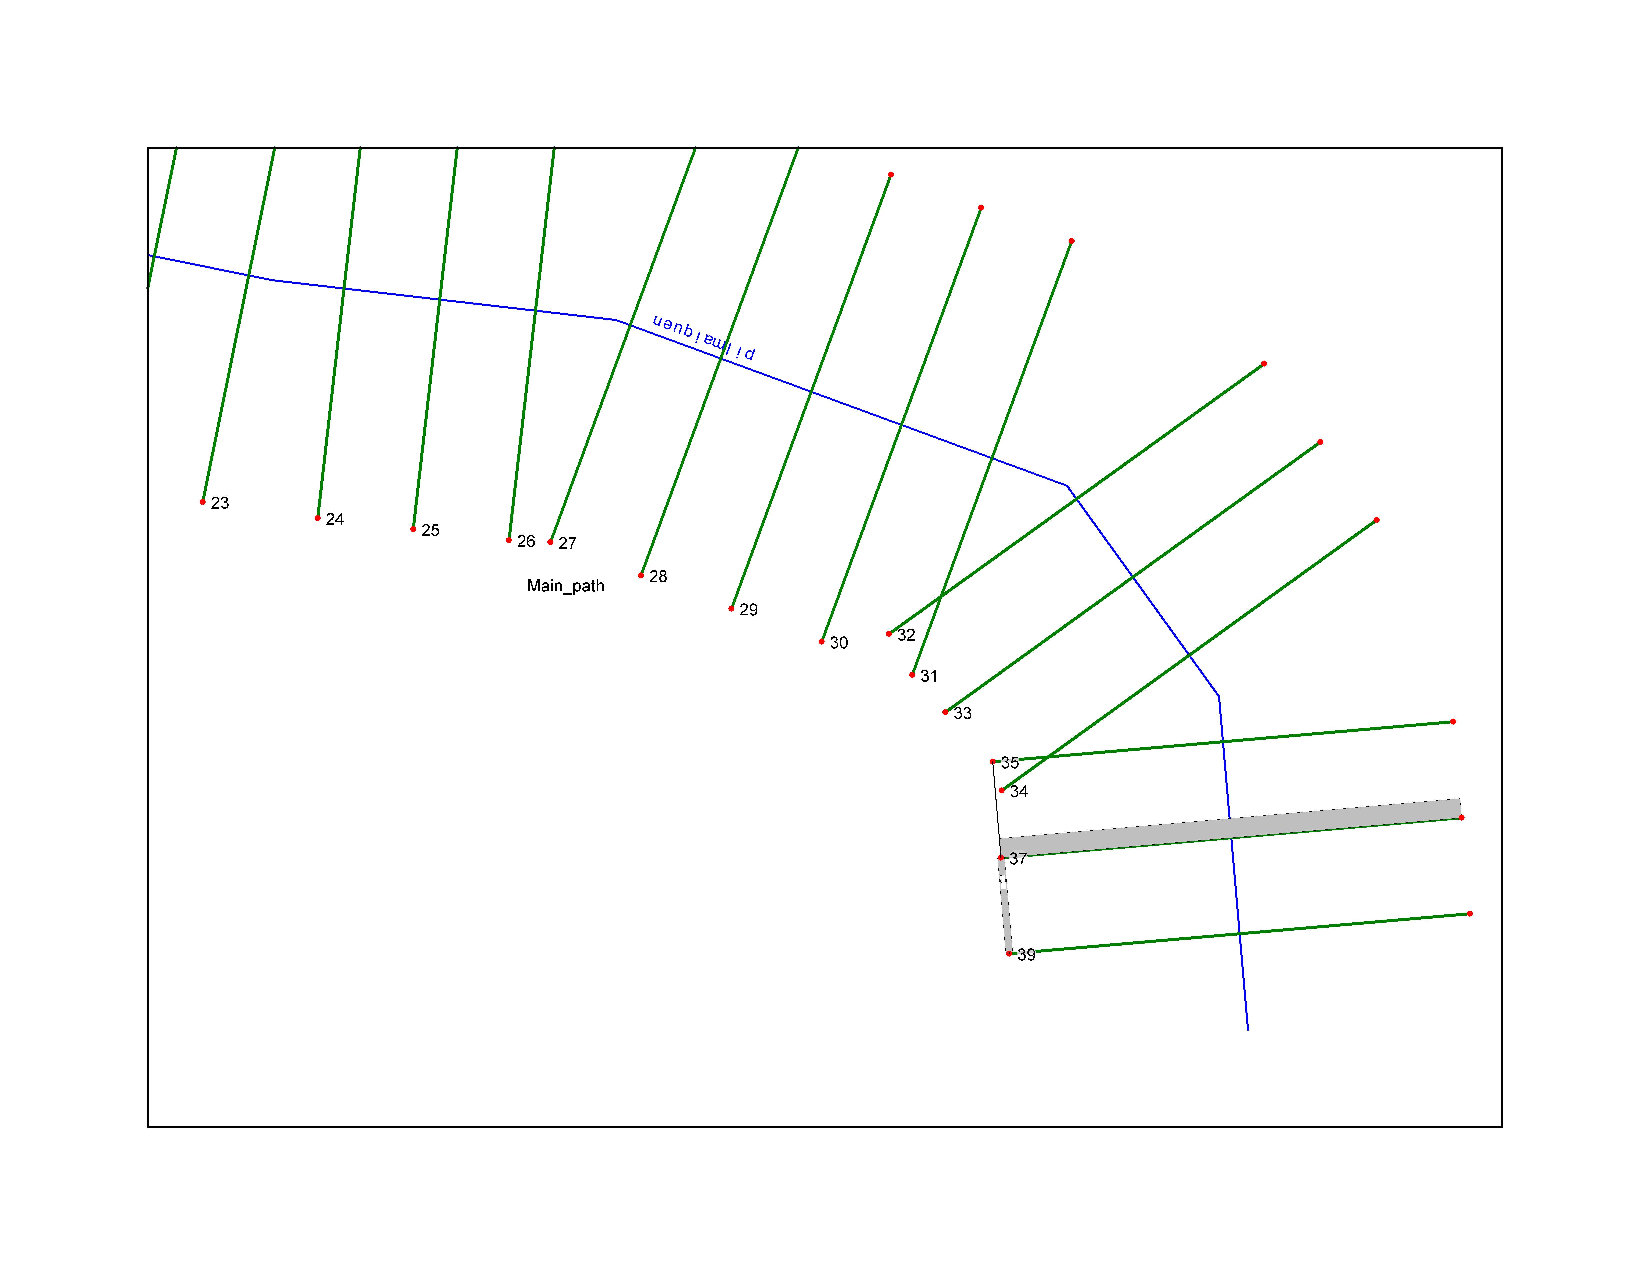
\includegraphics[width=0.6\linewidth]{imagenes/rio.pdf}
    \caption{Cortes transversales del río Pilmaiquén con el muro y las bocatomas incorporadas}
\end{figure}

Una vez lista la geometría, se procedió a correr la simulación con los periodos de retorno anteriormente mencionados. Dando los siguientes resultados:

\begin{figure}[H]
    \centering
    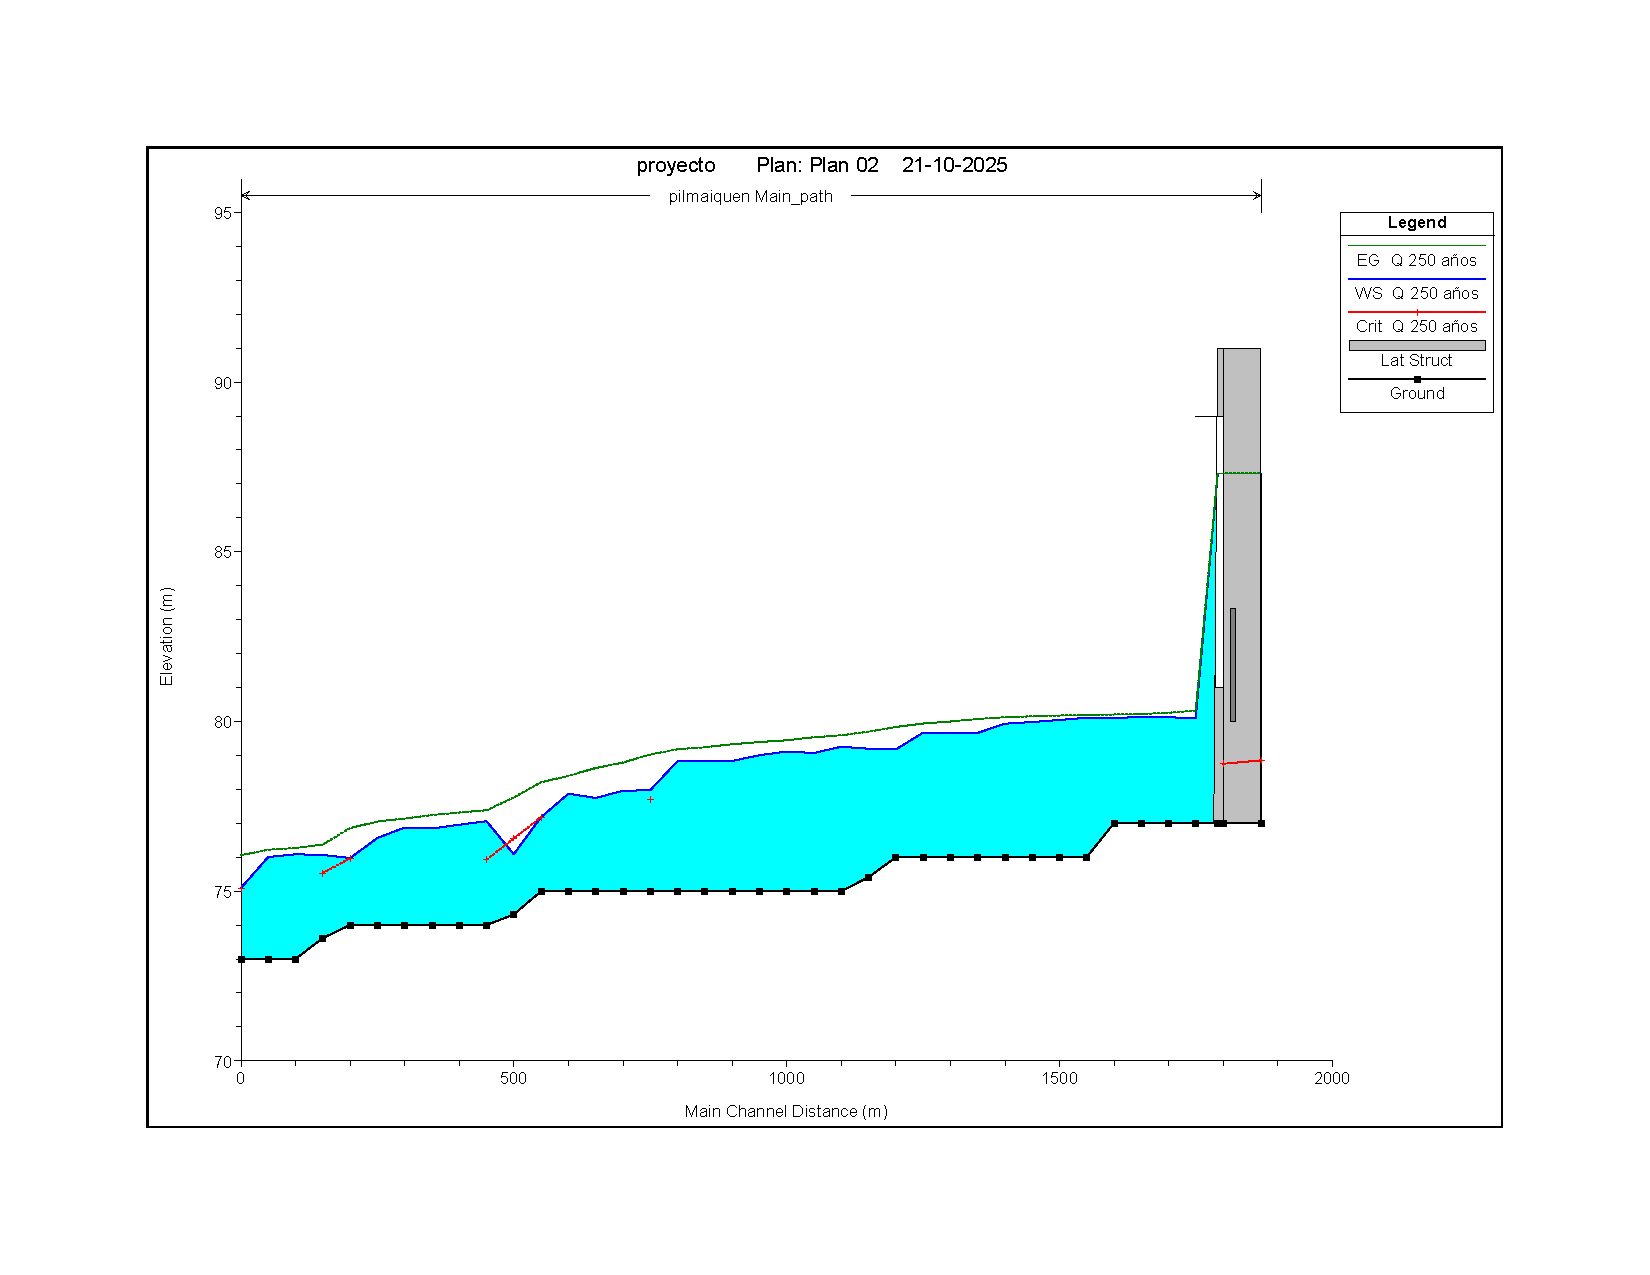
\includegraphics[width=0.6\linewidth]{imagenes/perfil_250_cb.pdf}
    \caption{Perfil hidráulico con caudal asociado a periodo de retorno de 250 años con muro y bocatomas}
\end{figure}

\begin{figure}[H]
    \centering
    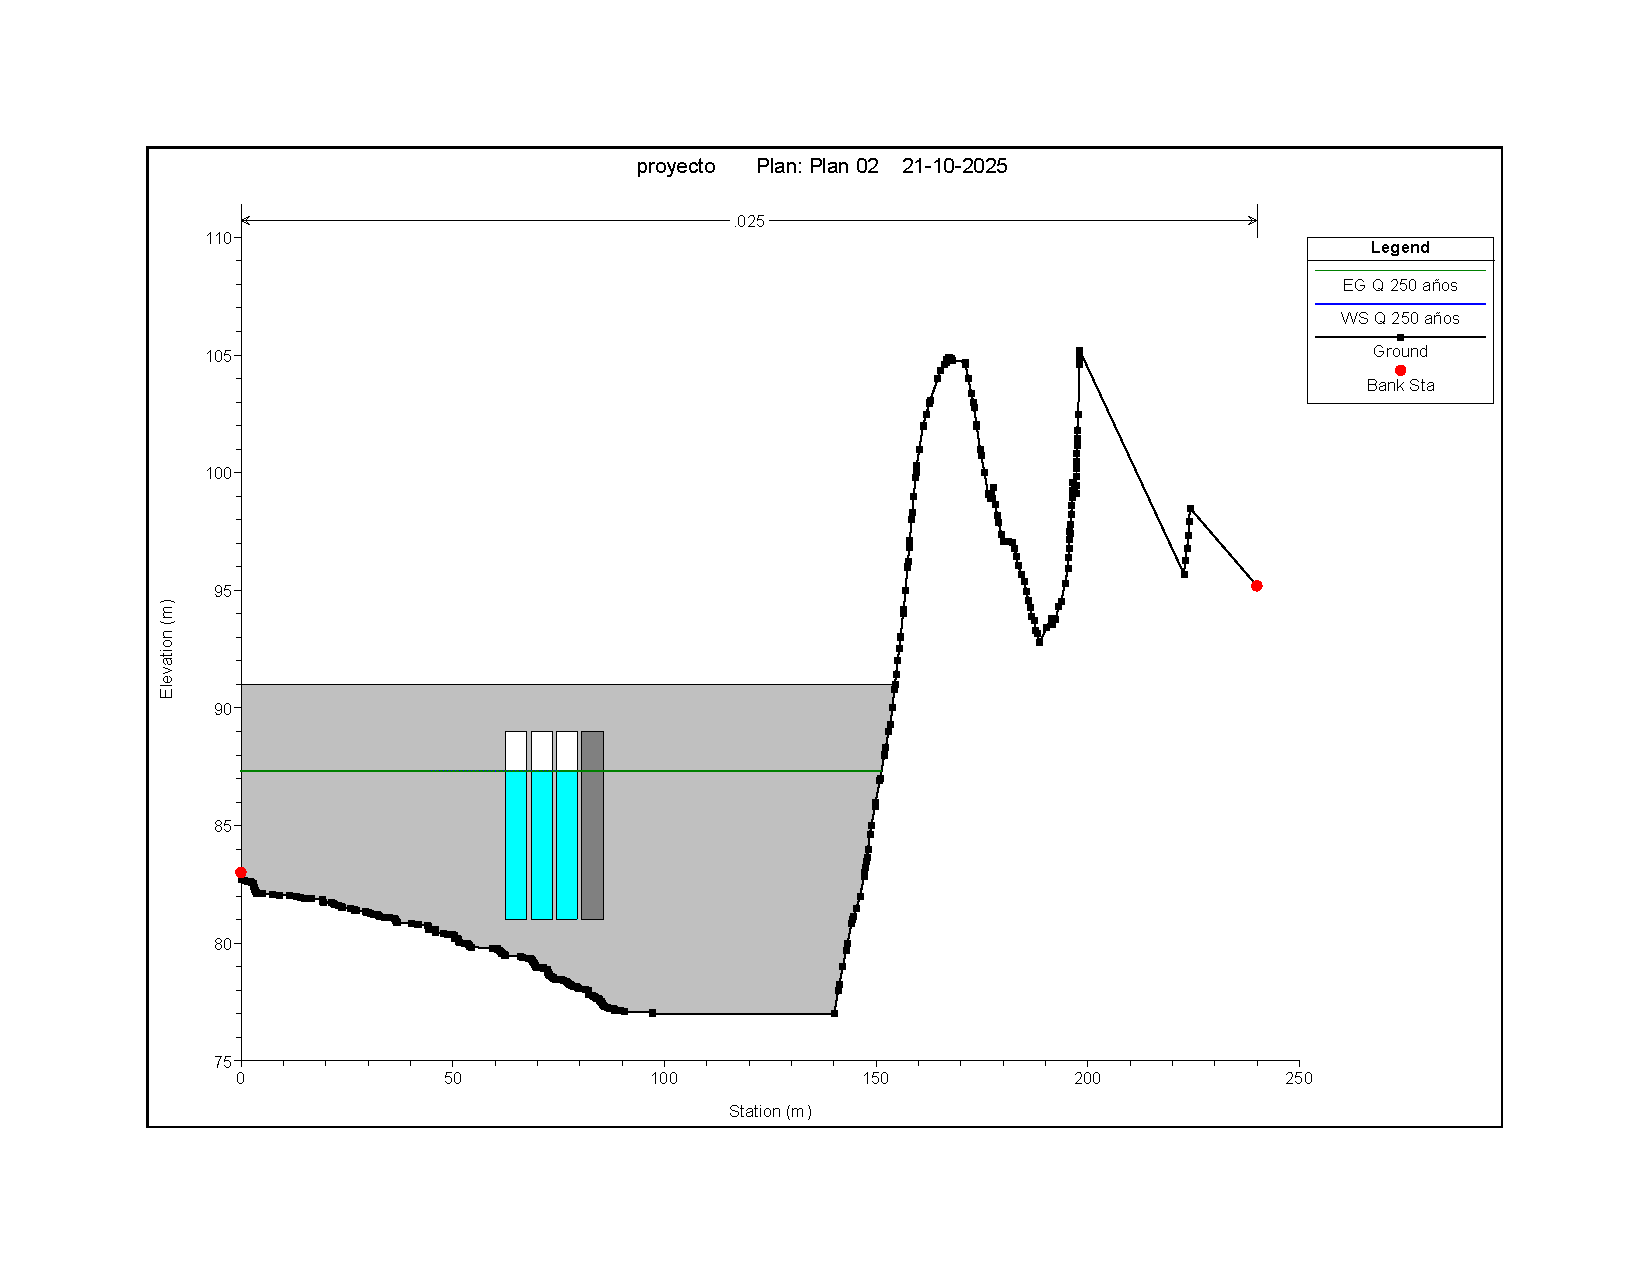
\includegraphics[width=0.6\linewidth]{imagenes/corte_250_cb.pdf}
    \caption{Corte transversal del río Pilmaiquén con muro y bocatomas para periodo de retorno de 250 años}
\end{figure}

\begin{figure}[H]
    \centering
    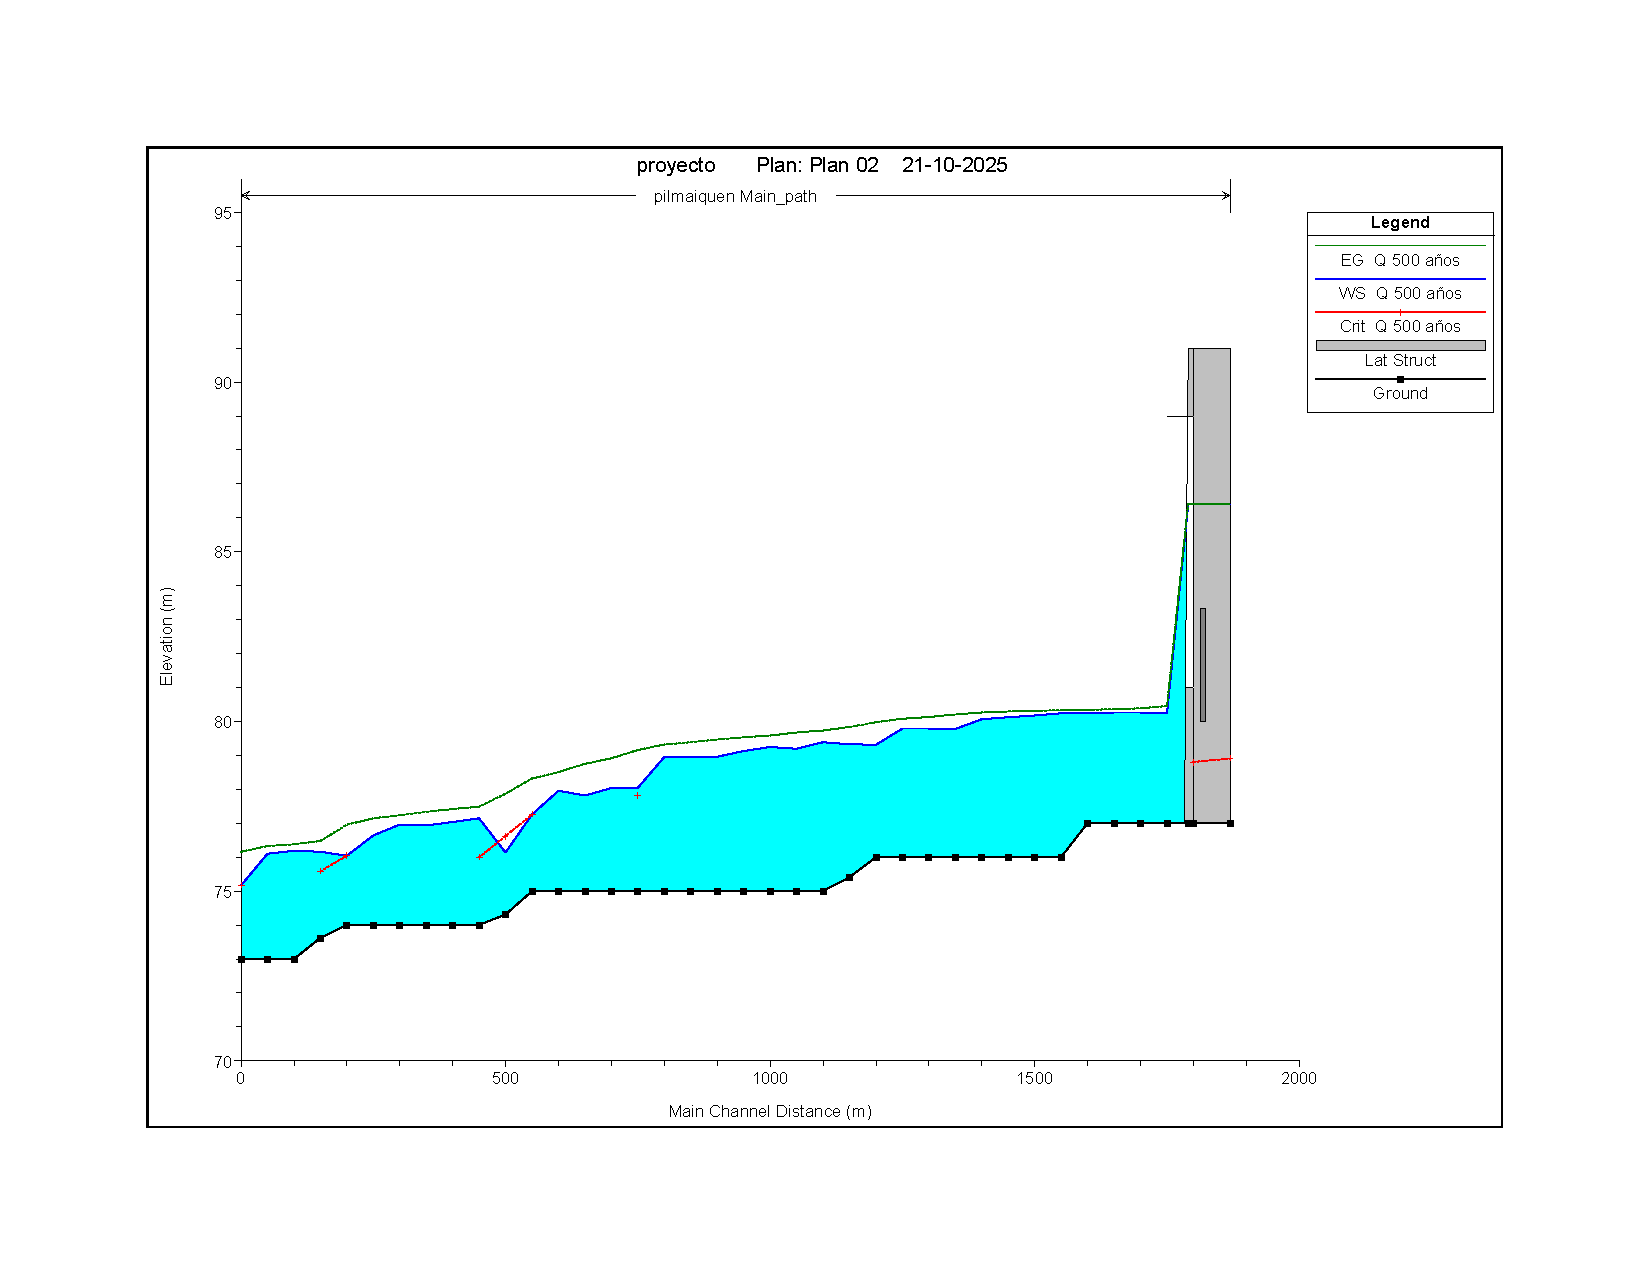
\includegraphics[width=0.6\linewidth]{imagenes/perfil_500_cb.pdf}
    \caption{Perfil hidráulico con caudal asociado a periodo de retorno de 500 años con muro y bocatomas}
\end{figure}

\begin{figure}[H]
    \centering
    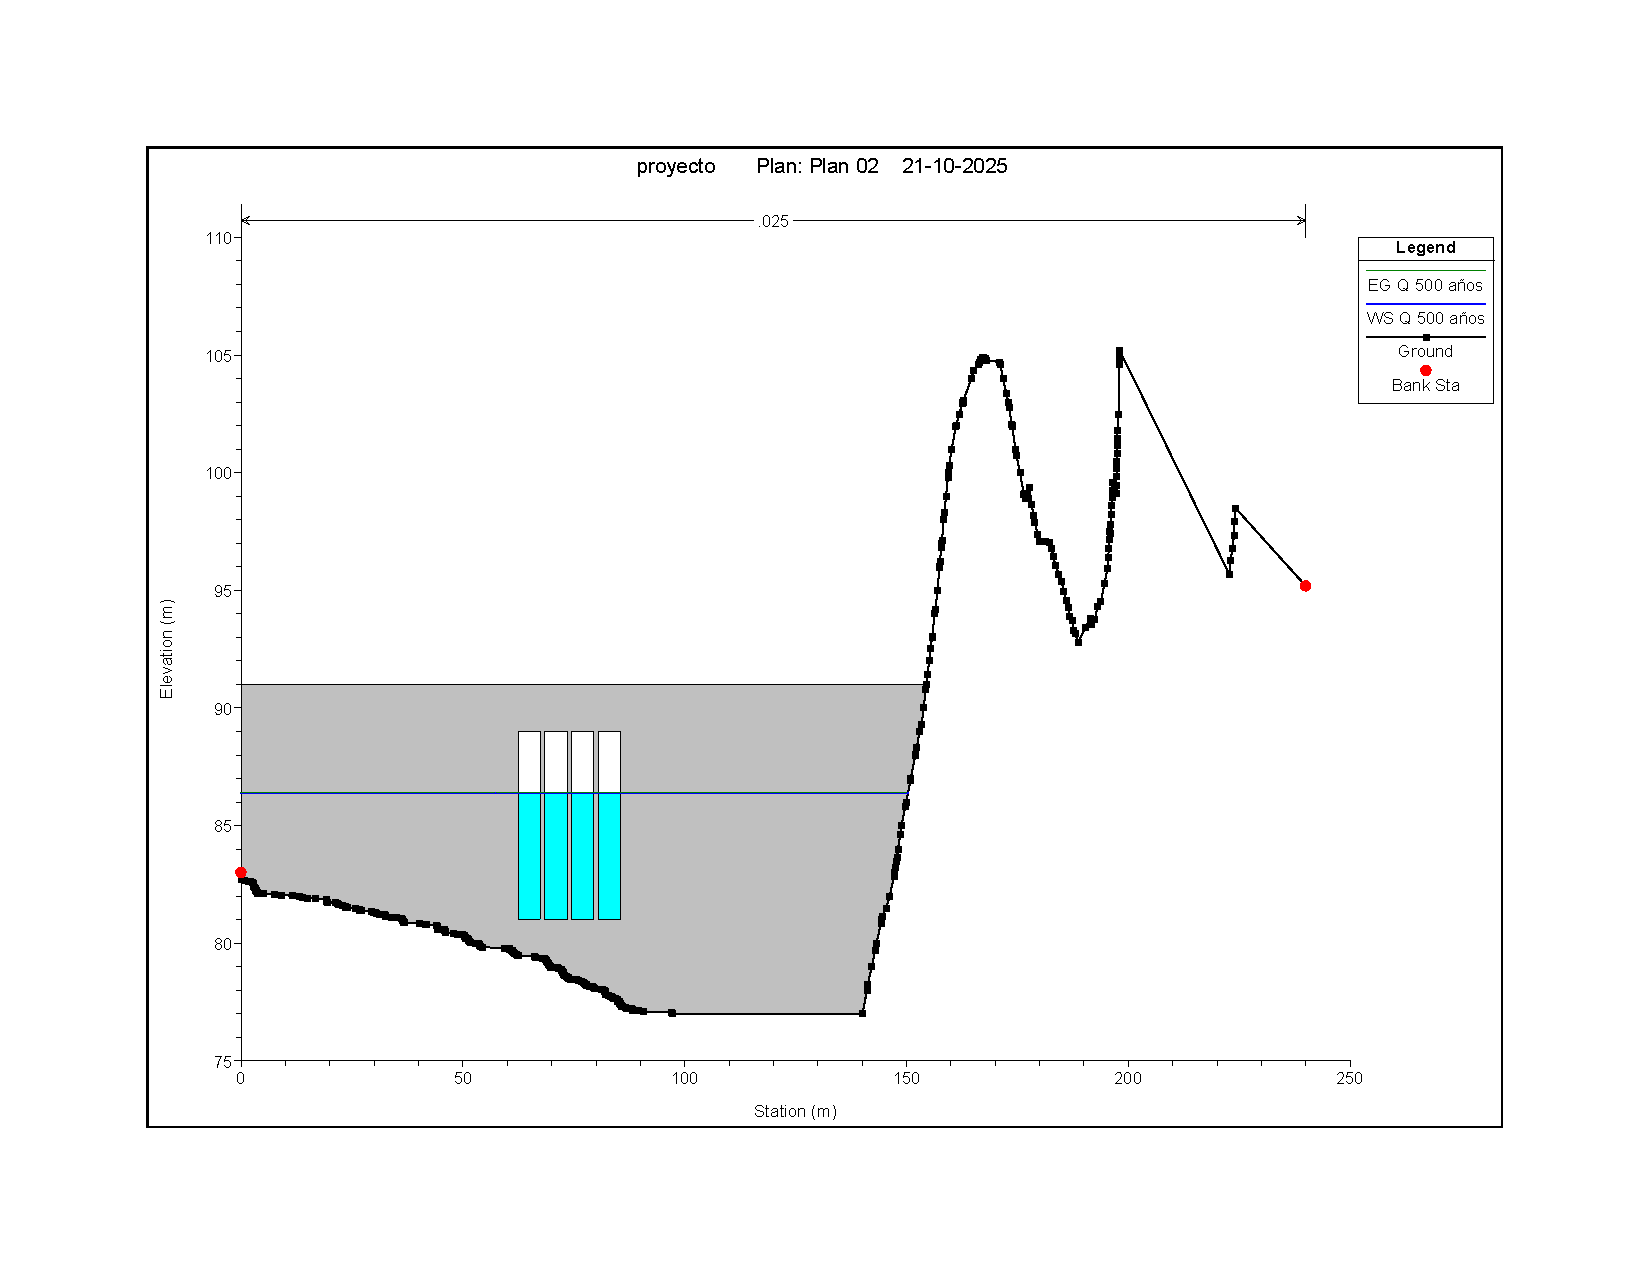
\includegraphics[width=0.6\linewidth]{imagenes/corte_500_cb.pdf}
    \caption{Corte transversal del río Pilmaiquén con muro y bocatomas para periodo de retorno de 500 años}
\end{figure}


\end{document}